\documentclass[conference]{IEEEtran}
\usepackage{longtable}
\usepackage{graphicx}
\usepackage{graphics}
\usepackage{float}
\usepackage{cite}
\usepackage{amsmath,amssymb,amsfonts}
\usepackage{algorithmic}
\usepackage{graphicx}
\usepackage{textcomp}
\usepackage{xcolor}
\usepackage{dblfloatfix}
\usepackage{cleveref}
% \usepackage{algpseudocode}
\usepackage{xcolor}
\usepackage[linesnumbered,ruled,vlined]{algorithm2e}

\title{Machine learning based metro edge computing network resource optimization algorithm for 5G and beyond applications}
\author{\IEEEauthorblockN{Luong Quoc Dat}
\IEEEauthorblockA{\textit{Dept. of Electrical Engineering} \\
\textit{Technical University of Eindhoven}\\
}}
\date{Feb 2021}

\makeatletter
\newcommand{\removelatexerror}{\let\@latex@error\@gobble}
\makeatother

%%% Coloring the comment as blue
\newcommand\mycommfont[1]{\footnotesize\ttfamily\textcolor{blue}{#1}}
\SetCommentSty{mycommfont}

\SetKwInput{KwInput}{Input}                % Set the Input
\SetKwInput{KwOutput}{Output}              % set the Output


\begin{document}
\maketitle

\begin{abstract}
Nowadays, there is a huge demand for optical metro network infrastructure in terms of service expectations for applications in 5G and beyond. In the real-life scenario with multiple applications and different user patterns for each application and different applications' latency requirements, a resource optimization algorithm should be developed to automate the application deployment in the optical network. This project aims to develop a reinforcement learning based algorithm to optimize the deployment of 5G and beyond applications in the optical metro network to satisfy applications’ requirements. In the first half part of the thesis, the real applications' deployment, user traffic pattern generation, set up an experiment to capture traffic from each application in the network and simulation software design are already achieved.
\end{abstract}

\section{Introduction}
\label{sec:Introduction}
% section Introduction (begin)
In recent years, it is undeniable that there is a significant increasing trend in the number of users as well as devices connected to the Internet \cite{International2017}. This trend leads to huge demands in optical metro networks infrastructure in terms of service expectations. Therefore, optical metro networks should efficiently support a variety of access applications with different dynamic user traffic patterns from various sources such as enterprises, home applications, media streaming, and IoT applications. These applications not only require high bandwidth demands but also require low latency response. For those latency-sensitive applications, cloud computing in data centers is not efficient enough to support because of the long distance between the data center and end-users, causing a long delay from signal propagation leads to high latency. To address this issue, edge computing where the computing servers have been brought to the edge near the end-users is a good solution \cite{Shi2016}.

Edge computing refers to the enabling technologies that allow computation to be performed at the metro network so that computing happens near data sources. It works on both downstream data on behalf of cloud services and upstream data on behalf of IoT services. Edge computing can be any computing or networking resource residing between data sources and cloud-based data centers. For example, in a metro network, an optical metro node can be equipped with powerful servers as edge computing and handle requests and responses between users and the cloud datacenters. In edge computing, the end device not only consumes data but also produces data. And at the network edge, devices not only request services and information from the cloud but also handle computing tasks including processing, storage, caching. Edge computing could yield many benefits. The most important benefit is reducing application latency. For instance, researchers built a proof-of-concept platform to run a face recognition application in \cite{7372286}, and the response time is reduced from 900 to 169 ms by moving computation from cloud to the edge. Researchers in \cite{5280678} also have shown that using edge computing to offload computing tasks for wearable cognitive-assistance systems improves response times by between 80 and 200 ms and reduces energy consumption by 30 to 40 percent.

In the TU/e lab, there is an optical metro ring network that has already been set up as we can see from Figure \ref{fig:full_metro_ring}, the ring optical metro network consists of 4 nodes connected by 10Gbps optical links. In a real-life scenario, the traffic that comes from the access network will be aggregated to the metro network. There are also optical links to the data center that have been set up in the lab.

\begin{figure}[]
    \centering
        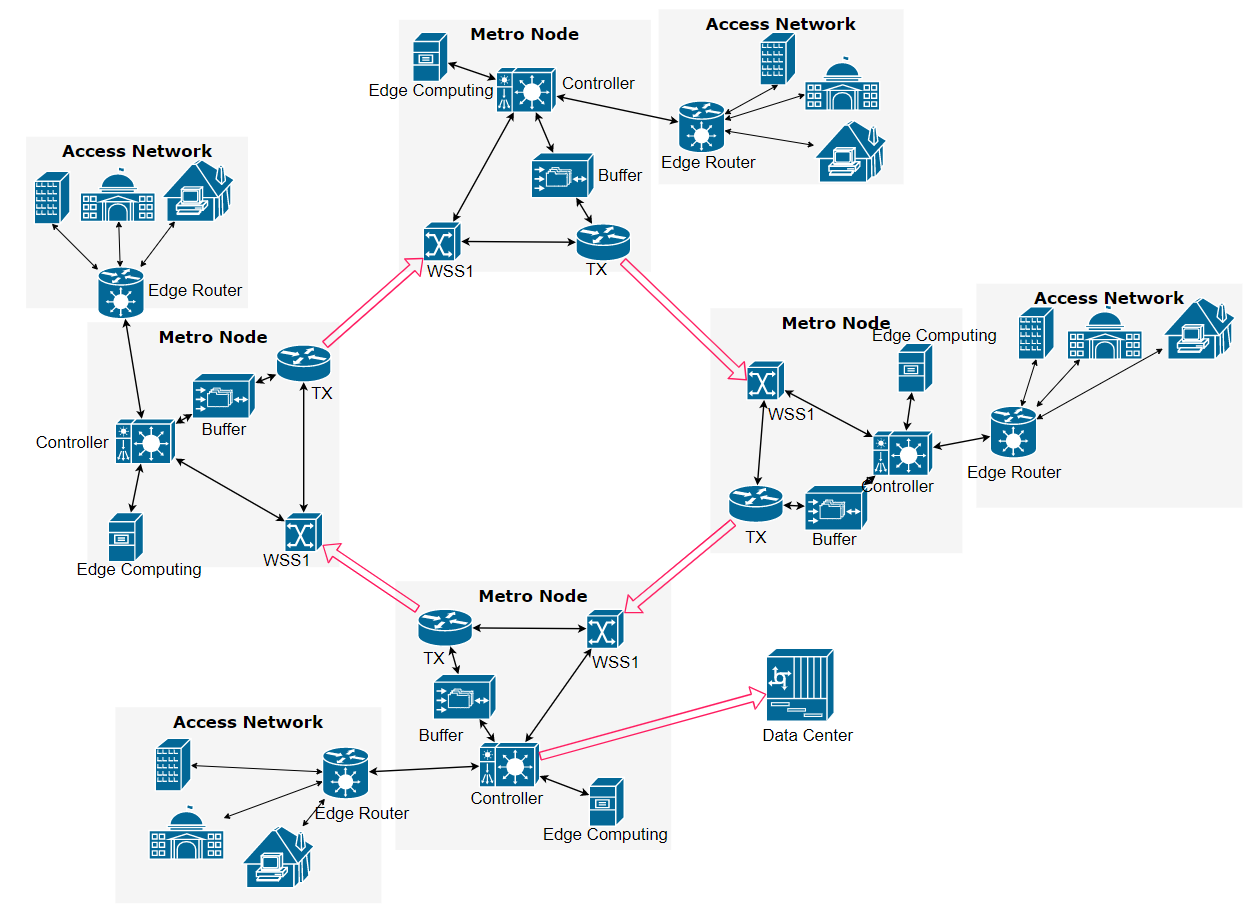
\includegraphics[scale = 0.25]{imgs/metro_ring_with_DC.png}
        \caption{Metro Ring Network}
        \label{fig:full_metro_ring}
    \end{figure}

Bitao \textit{et. al.} in \cite{8818041} demonstrated serving new applications in optical metro access ring network with edge computing resource using software defined networking (SDN) reconfiguration and network slicing (NS). The result shows that the latency for a latency-sensitive application would remain low and satisfy the application requirements. However, if the load on the link increase due to the bandwidth-intensitive application, the latency of the latency-sensitive application could raise and not meet the application requirement. It also pointed out that, to solved the problem, the potential solution could be to reallocate the destination of the latency-insensitive application to save bandwidth for the latency-sensitive application. In the real-life scenario with multiple applications and different user patterns for each application and different applications' latency requirements, a resource optimization algorithm should be developed to automate the application deployment in the optical network. 

The traditional simple traffic classification using TCP or UDP headers proved to be not capable of when dealing with the high complexity problem \cite{4738466}. In recent years,  Machine learning (ML) has been explored as a bright candidate to deal with the problem in the optical network including resource allocation to optimize the network by using Reinforcement Learning (RL) \cite{Gu2020}. 

Based on it, this project aims to develop a reinforcement learning based algorithm to optimize the deployment of 5G and beyond applications in the optical metro network to satisfy applications’ requirements.
To achieve the thesis objective, the project has the following main tasks:
\begin{itemize}
    \item Deploy real-life applications in the optical network.
    \item Develop user traffic generation model for each application.
    \item Set up an experiment to collect traffic data in the metro ring network.
    \item Develop network simulation model based on data collected in the experiment.
    \item Apply and train reinforcement learning model with simulation.
    \item Train the reinforcement learning model in the optical metro network.
\end{itemize}

In the first half part of the thesis, the real applications' deployment, user traffic pattern generation, set up an experiment to capture traffic from each application in the network and simulation software design are already achieved. 

The rest of this report is structured as follows. The related work is presented in section \ref{sec:Literature review} while the real application deployment, user traffic generation and traffic capture are presented in section \ref{sec:Application Deployment} and section \ref{sec:User traffic generation}, respectively. The simulation design is represented in section \ref{sec:Simulation} meanwhile, in the last section \ref{sec:Plan}, the plan for the second part of the thesis is discussed. 

% section Introduction (end)

\section{Literature review}
\label{sec:Literature review}
% section Literature review (begin)

According to Danish Rafique \textit{et. al.} in \cite{Rafique:18}, the main motivations to apply ML method in the optical network are heterogeneity, reliability, capacity, and complexity, which are not suitable with the static traditional design principle anymore. The author also argued that network self-configuration, including resource allocation and service (re)configurations—both for physical and virtual infrastructure are among the core application of RL, which is a branch of ML, in optical network. Applying Machine Learning, especially Reinforcement Learning in optical network is not new. Researchers have been using RL for path selection and wavelength selection in optical burst switched networks since 2007 \cite{4395244}. They proposed algorithms based on Q-learning to solve these problems near-optimally. In \cite{8873660}, Pham Tran Anh Quang \textit{et. al.,} also using reinforcement learning to deal with the allocation of virtual network functions (VNFs) for realizing network services. The author proposed reinforcement learning with a neural network, which is called deep reinforcement learning (DRL), and "memory play" which allows having the advantages of supervised learning to allocate VNFs in the network.

Briefly speaking, reinforcement learning deals with learning via interaction and feedback, or in other words learning to solve a task by trial and error, or acting in an environment and receiving rewards for it. Basically, as we can see from Figure \ref{fig:RL_overview}, the agent is the learner and the decision-maker from the environment, where the agent learns and decides what actions to perform. An action belongs to a set of actions that the agent can perform and the state is the state of the agent in the environment. For each action selected by the agent, the environment provides a reward which usually is a scalar value. The Policy is the decision-making function (control strategy) of the agent, which represents a mapping from situations to actions.

\begin{figure}[]
\centering
    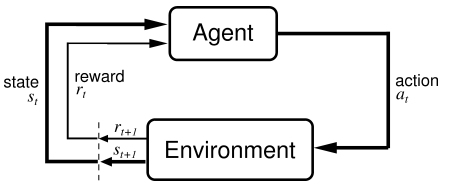
\includegraphics[scale = 0.7]{imgs/DRL.png}
    \caption{Agent-environment interaction}
    \label{fig:RL_overview}
\end{figure}

Reinforcement Learning has several more techniques to offer. To name a few, there are Deep Deterministic Policy Gradient (DDPG), Proximal Policy Optimization (PPO), Actor-Critic, and the most well-known reinforcement learning technique Double Deep Q Network (DDQN) \cite{Mnih2015}. In this work, DDQN is a bright candidate to use in this thesis not only because it has high efficiency but also based on the fact that the environment action space in this work is discrete. Besides, it is a well-built algorithm with high support from various tools and libraries.

% section Literature review (end)


\section{Application Deployment}
\label{sec:Application Deployment}
% section Application Deployment (begin)

There are many usage cases of edge computing in real-life represented in various papers \cite{International2017, 7469991, Shi2016}. Among the applications that could be deployed in the optical metro network, web searching, web serving, and online shopping are chosen. They used the most popular platform on the Internet today: Nginx server, which has taken from Apache since April 2019 \cite{netcraft_news_2021}. To deploy all these real application servers to the optical metro network, we have 2 options: container and virtual machine (VM). In this work, all the applications are deployed using docker container technology. 

A container is a standard unit of software that packages up code and all its dependencies so the application runs quickly and reliably from one computing environment to another. A Docker container image is a lightweight, standalone, executable package of software that includes everything needed to run an application: code, runtime, system tools, system libraries, and settings. Containers and virtual machines have similar resource isolation and allocation benefits but function differently because containers virtualize the operating system instead of hardware. Containers are more portable and efficient \cite{7036275}.

Containers are an abstraction at the app layer that packages code and dependencies together. Multiple containers can run on the same machine and share the OS kernel with other containers, each running as isolated processes in userspace. As in Figure \ref{fig:container_img}, containers take up less space than VMs (container images are typically tens of MBs in size), can handle more applications, and require fewer VMs and Operating systems \cite{docker}.

\begin{figure}[]
    \centering
        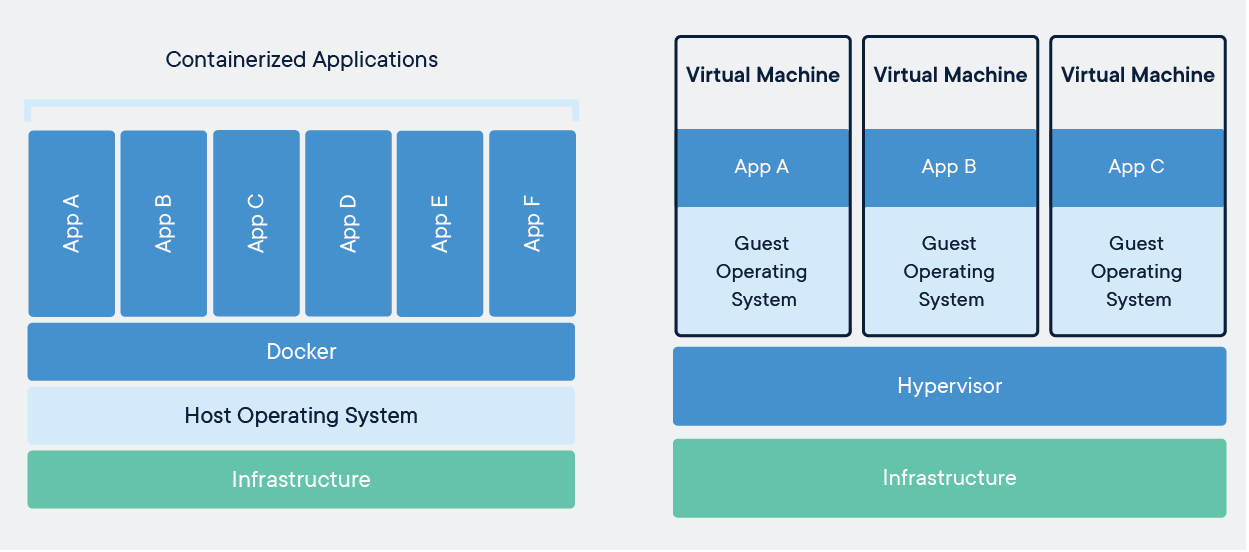
\includegraphics[scale = 0.25]{imgs/container-VM.png}
        \caption{Container and Virtual Machine}
        \label{fig:container_img}
    \end{figure}

The application servers can be deployed in any node in the network. Because the access network is not available in the lab, simulated traffic is generated from the server in each node to the metro network as user simulator containers. Both application servers and users for each application server are containerized in docker containers as in Figure \ref{fig:real_set_up}.

\begin{figure}[]
\centering
    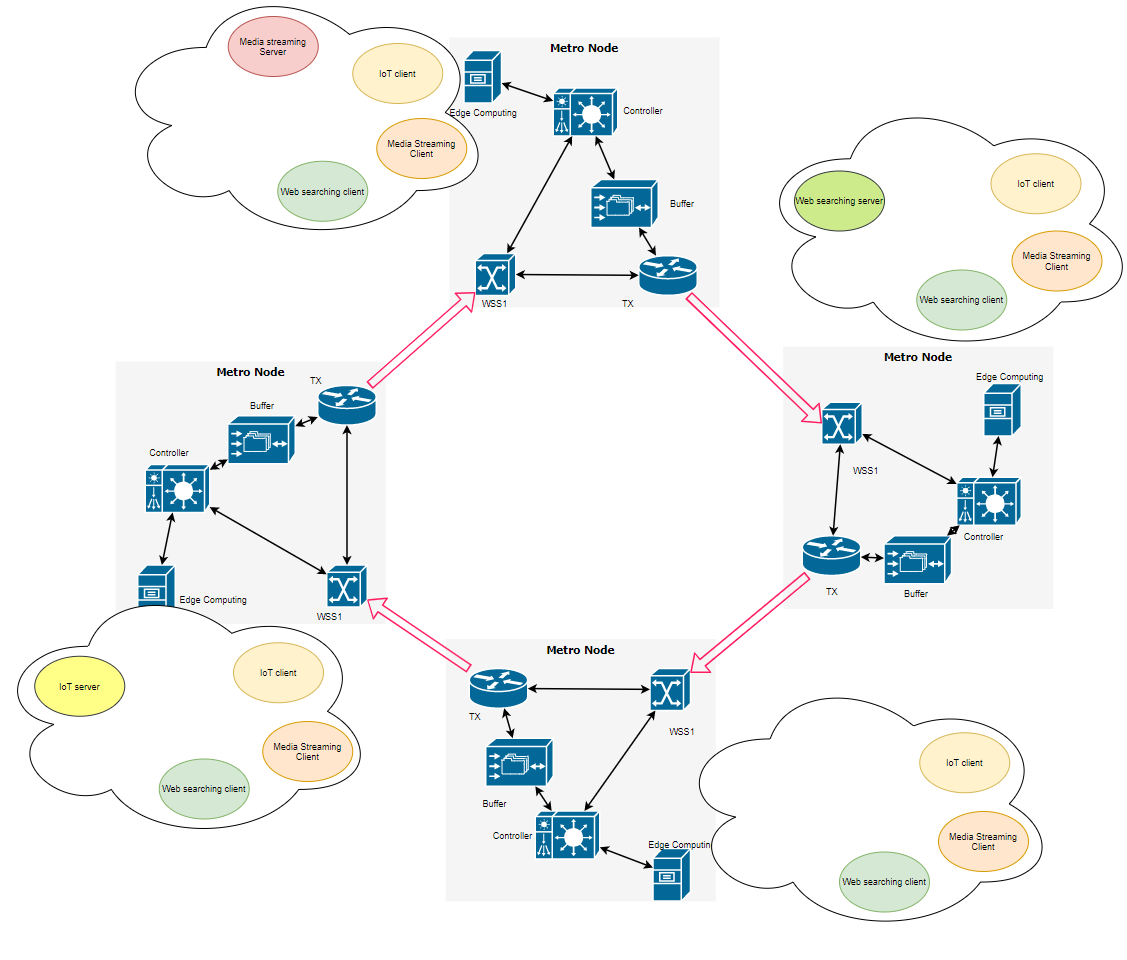
\includegraphics[scale = 0.3]{imgs/real_experiment_set_up.png}
    \caption{Metro Ring Network}
    \label{fig:real_set_up}
\end{figure}

To build an effective algorithm that determines which node each application server should be, the bandwidth that each application server occupies based on real user requests is captured. To capture the traffic between each application and its user, node 3 and node 4 have been used to experiment as we can see in Figure \ref{fig:server_deployment}. In the experiment, we captured each application at a time.

In the media streaming server, an HD video 1080p resolution length of 5.15 minutes is stored in the Nginx server and ready to be requested from the user simulator. Similarly, for web serving, web searching, and online shopping, there is a website page of Wikipedia, google result page and amazon frontpage HTML file is stored inside the Nginx server, respectively.

\begin{figure}[]
    \centering
        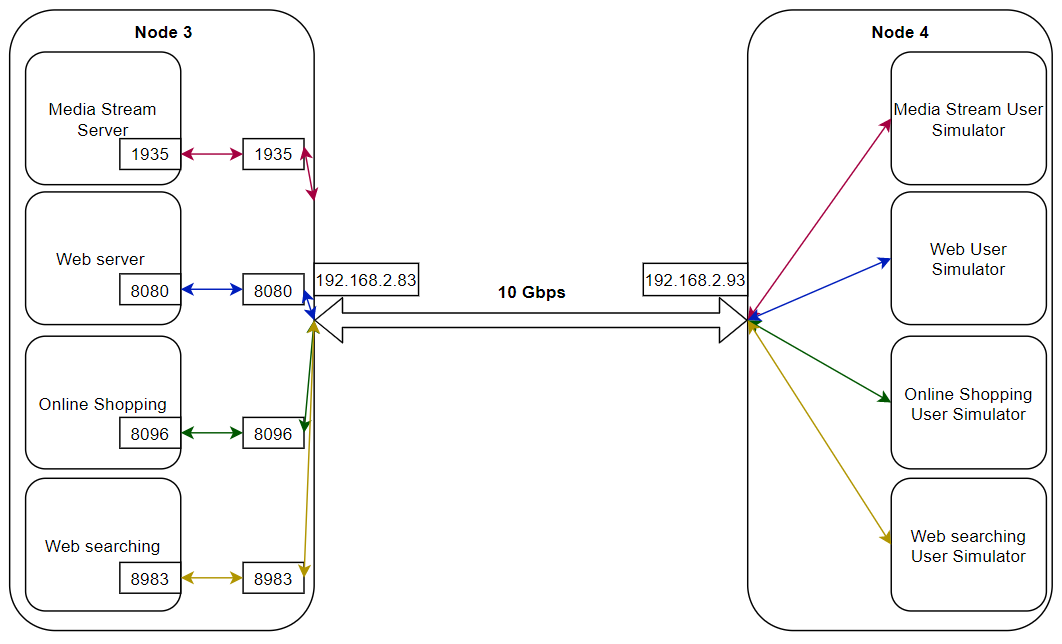
\includegraphics[scale = 0.3]{imgs/server_deployment.png}
        \caption{Application and client Containers in node 3 and 4}
        \label{fig:server_deployment}
    \end{figure}

% section Application Deployment (end)


\section{User traffic generation and traffic capture}
\label{sec:User traffic generation}
% section User traffic generation (begin)
 
To the most knowledge of the author, most of the user behavior can be assumed daily periodic based on research papers \cite{Kooti2016,Ullah2012,Taghavi2012,Yu2006}. Based on the patterns in these researches, a software program python-based has been constructed to simulate the user. To simulate multiple concurrent users at the same time we used multi-threading in python. Each thread represents a user. The algorithm to generate users for each application is represented in Algorithm \ref{algo:user-traffic-gen}. 

For each different server application, we used different tools to make user requests. For media streaming (Nginx server), RTMP protocol and FFmpeg has been used to send request from each user thread. For web searching, web serving, and online shopping, the user requests are HTTP protocol and python packages for HTTP requests have been used.

\removelatexerror
\begin{algorithm}[]
    \DontPrintSemicolon
        \KwInput{\begin{itemize}
            \item Number of concurrent active users hourly in 1 day.
            \item Scale ratio for each day.
        \end{itemize}}
        \KwOutput{User threads hourly}
        
        User thread:
        \While {True}
        {
            Send a request to the server.

            Sleep(Read/watch duration)
        }

        Initial: Create an initial number of user threads based on 1st day.

        \For{each day in our simulation time}
        {
            \For{each hour in a day}
            {
                \While {runtime less than an hour}    
                {
                    $UserNumber = UserNumberThisHour + (UserNumberNext Hour - UserNumberThisHour)*runtime/hour$
                    $UserNumber = UserNumber*scale$

                    \If{$UserNumber > CurrentNumber$}
                    {
                        create $UserNumber - CurrentNumber$ threads.
                    }
                    \Else
                    {
                        stop and remove $CurrentNumber - UserNumber$ threads.
                    }
                    Sleep(1 minute)
                }
            }
        }
    \caption{User request generator}
    \label{algo:user-traffic-gen}
\end{algorithm}

According to \cite{5GPPP2020}, around 70\% traffic should be from video streaming applications, 30\% for other applications. Here, in this work, 30\% is divided equally among 3 other applications: web serving, web searching, and online shopping. The number of users should be used to stress the server for each application is calculated based on the traffic on the link that each application generated and based on the ratio above.

\begin{figure}[]
    \centering
        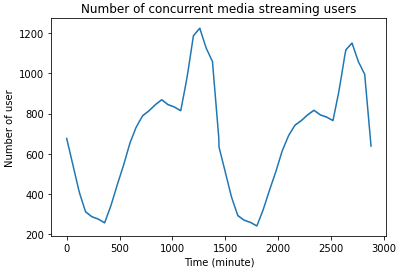
\includegraphics[scale = 0.8]{imgs/media_streaming_concurrent_user_2days.png}
        \caption{Media user generated from user simulation}
        \label{fig:media_user}
    \end{figure}

\begin{figure}[]
    \centering
        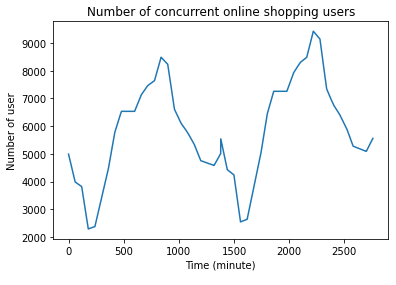
\includegraphics[scale = 0.8]{imgs/online_shopping_concurrent_users_2days.png}
        \caption{Online Shopping user generated from user simulation}
        \label{fig:shopping_user}
    \end{figure}

\begin{figure}[]
    \centering
        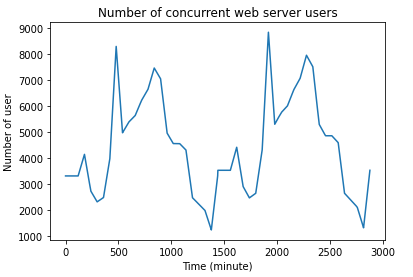
\includegraphics[scale = 0.8]{imgs/web_server_concurrent_user_2days.png}
        \caption{Web server user generated from user simulation}
        \label{fig:webServinguser}
    \end{figure}

\begin{figure}[]
    \centering
        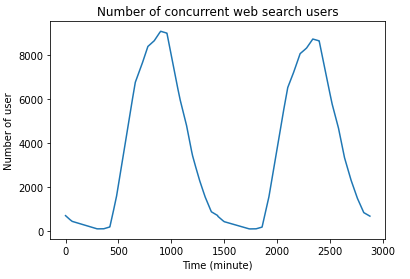
\includegraphics[scale = 0.8]{imgs/web_search_concurrent_users_2days.png}
        \caption{Web searching user generated from user simulation}
        \label{fig:webSearching_user}
    \end{figure}

NetData \cite{netdata} has been used to capture the traffic on the link with a sampling rate of 1 second. All the application traffic traces has been captured as in Figure \ref{fig:all_app_resp},\ref{fig:media_resp},\ref{fig:shopping_resp},\ref{fig:search_resp},\ref{fig:serving_resp}. 

\begin{figure}[]
    \centering
        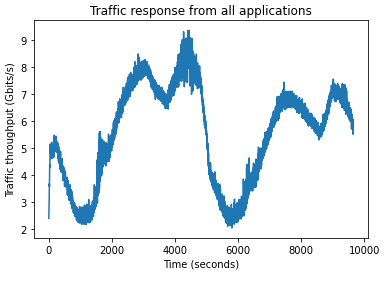
\includegraphics[scale = 0.8]{imgs/agrregated_traffic_all_apps.png}
        \caption{Traffic response from all applications}
        \label{fig:all_app_resp}
    \end{figure}

\begin{figure}[]
    \centering
        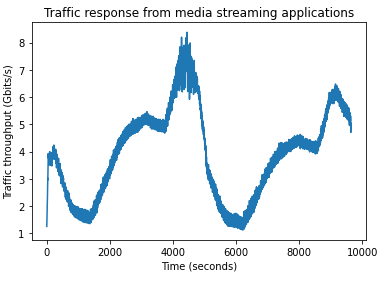
\includegraphics[scale = 0.8]{imgs/media_streaming_response_24_02.png}
        \caption{Traffic response from media streaming application}
        \label{fig:media_resp}
    \end{figure}

\begin{figure}[]
    \centering
        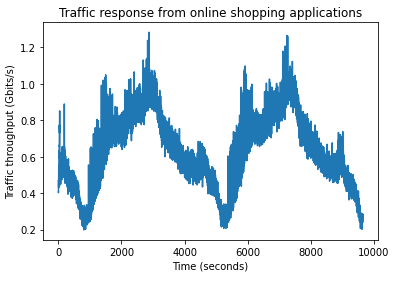
\includegraphics[scale = 0.8]{imgs/online_shopping_response.png}
        \caption{Traffic response from online shopping application}
        \label{fig:shopping_resp}
    \end{figure}

\begin{figure}[]
    \centering
        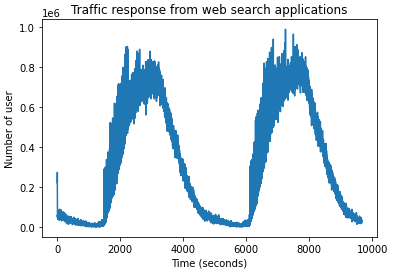
\includegraphics[scale = 0.8]{imgs/search_server_response.png}
        \caption{Traffic response from web search application}
        \label{fig:search_resp}
    \end{figure}

\begin{figure}[]
    \centering
        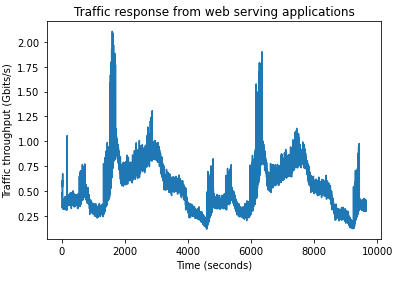
\includegraphics[scale = 0.8]{imgs/web_server_response.png}
        \caption{Traffic response from web server application}
        \label{fig:serving_resp}
    \end{figure}

% section User traffic generation (end)

\section{Simulation}
\label{sec:Simulation}
% section Simulation (begin)

To simulate the optical metro network with edge computing attached to each node and applications as well as client containers in each edge computing, the author proposes a simulation model which combines a network simulator based on OMNET++ and python programming. The optical communication links, buffers, TXs, and WSSs are modeled using the OMNET++ library. Meanwhile, the edge computing server which contains application servers and client containers is modeled using python. 

%TODO: Add a picture to show how the simulation works.

\subsection{OMNET++ software simulator}
OMNeT++ is an extensible, modular, component-based C++ simulation library and framework, primarily for building network simulators \cite{andras_rudolf}.

Briefly speaking, in this OMNET++ software, during the initial stage, the control packets are sent to establish the time slot in the whole network. The control packets contain a table of the destinations of packets in their time slot. In the running stage, the sources generate the data packets based on pre-defined load parameters to buffer with specify the destination of each packet. The buffers store the data packets from sources in their buffers and then check which wavelength is available and assign the data packet from the most loaded buffer to the available wavelength. In the meantime, the buffer also updates the control packet based on the destination of the data packet. If the buffers are full, the packet from the source would be discarded. The combiner is used to combine the packets from WSS1 and buffer together and put them to the link, which would introduce 100us latency since the optical link is 20km long. The WSS1 in each node checks the control packet if the data packet coming in that time slot is belongs to the node or not. If the packet does not belong to the node, then the WSS1 just forwards it to the combiner to send it to another node. Otherwise, WSS1 drops the packet to the node and calculates the latency of the packet.

\subsection{Python}

As we can see in Figure \ref{fig:simulation_software}, the OMNET++ is running inside the python program. For each specific time, the simulation program will take an action set from the control algorithm. The action can be to deploy a new application to the network or reallocate an application in the network. Based on the action, the applications are deployed accordingly as traffic sources in each node in the OMNET++ simulation program. The load parameter for each traffic source is calculated based on the experiment result in section \ref{sec:User traffic generation} for each specific time. The users' request traffics are deployed as user traffic sources in every node for each application. The load traffic from each application to its client is split based on the load requests from each client to the server. After preparing all the traffic source loads for server and client, the simulation program will use the bash command to run OMNET++ software to do the simulation with specific source loads parameters. After each iteration, the latency, total packet arrival, and packet lost parameter are captured and sent to the control algorithm.

\removelatexerror
\begin{algorithm}[]
    \DontPrintSemicolon
        
        \KwInput{Deployment Action}
        \KwOutput{Network Performance metrics}
        \KwData{Traffic data}

        \For{each data in traffic data}
        {
            \For{each application in deployment action}
            {
                \If{Application is not created yet}
                {
                    Create an application with a particular index.
                }
                \If{Application already belongs to the assigned node or Application does not belong to any node in the network or Assigned node resources is full}
                {
                    continue - skip the rest of this loop.
                }
                \If{Application currently belongs to another node}
                {
                    Delete the application in that node.
                }

                Deploy the application to the assigned node.

                Deploy users to other nodes.

            }

            Update the source list in each node.

            Create a .ini file from the source list in each node.

            Run OMNET++ software program.

            \If{simulation runtime greater than 10 min}
            {
                Return runtime error.
                
                Stop OMNET++ simulation
            }
            \Else
            {
                Return latency, packet arrival number, packet lost.
            }
        }
    \caption{Simulation Software}
    \label{algo:simulation-python}
\end{algorithm}

\begin{figure}[]
    \centering
        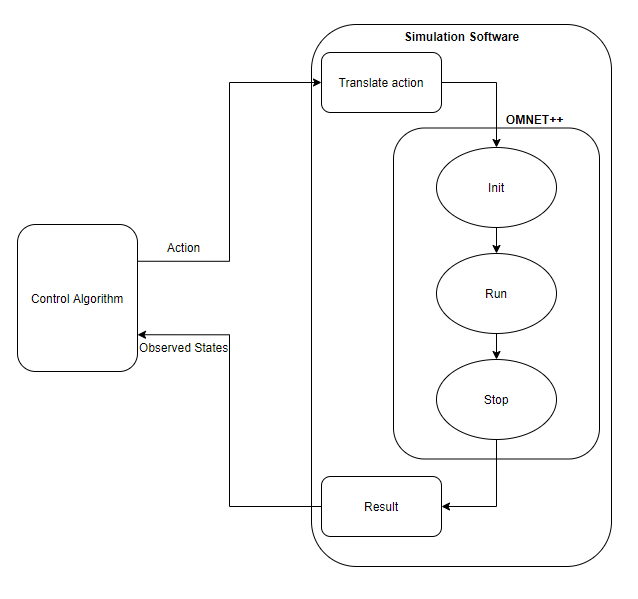
\includegraphics[scale = 0.5]{imgs/Simulation_software.png}
        \caption{Simulation model for each iteration}
        \label{fig:simulation_software}
    \end{figure}

% section Simulation (end)

\section{Network Modeling}
\label{sec:Network Modeling}
% section Network Modeling (begin)

We have $G = <V,L>$ with $ v \in V$ and $ l \in L $ 

% section Network Modeling (end)

\section{Conclusion}
\label{sec:Conclusion}
% section Conclusion (begin)

In conclusion, for the first part of the thesis. The following main tasks have been achieved: 
\begin{itemize}
    \item Deploy real-life applications in the optical network.
    \item Develop user traffic generation model for each application.
    \item Set up an experiment to collect traffic data in the metro ring network.
    \item Develop network simulation model based on data collected in the experiment.
\end{itemize}

The real-life applications that have been deployed are media streaming, web serving, web searching, and online shopping. The user pattern generator for each application also has been developed and tested with real-life applications. The result is shown in section \ref{sec:User traffic generation}. The traffic responses from server applications show that there is a similarity with the user request patterns. The simulation model is already developed based on the real experiment set up with 4 nodes and the source load parameters in each node are depend on the traffic capture in the experiment.

% section Conclusion (end)


\section{Plan}
\label{sec:Plan}
% section Plan (begin)
For the upcoming months, there are several tasks needed to be done.
\begin{itemize}
    \item Apply reinforcement learning algorithm and train with the simulation model.
    \item Automate the network with docker swarm or K8s and monitoring latency.
    \item Train the reinforcement learning model in the optical metro network.
\end{itemize}

\paragraph{Algorithm}
As we discussed in section \ref{sec:Literature review}, the bright algorithm to try should be DDQN but the other algorithm such as Actor-Critic also should be considered because of the fast training speed and the main limitation of DDQN is long convergence time \cite{article}. 

\paragraph{Application deploy automation and monitoring latency}
To automate the deployment and manage all applications, an orchestrator tool for the container should be used. Kubernetes (K8s) and Docker swarm are the two biggest players in this field. In the next part of the work, one of them should be used. Since NetData can not give the metrics about the latency of each container, we need another tool to monitor the latency. Prometheus is a good choice to do this. 

\paragraph{Online trainning}
After finalizing the algorithm, test with simulation, and automate the application deployment, the algorithm should be trained with the real-life scenario in the optical network. 
Ok TEst!

% section Plan (end)

\bibliographystyle{IEEEtran}
\bibliography{ref/refs.bib}

\end{document}
